\documentclass[11pt]{article}

\newcommand{\cnum}{ECE M146}
\newcommand{\ced}{Spring 2025}
\newcommand{\ctitle}[4]{\title{\vspace{-0.5in}\cnum, \ced\\Homework Set #1: #2}\author{\vspace{-0.35in}\\Name: #3, UID: #4}}
\usepackage{enumitem}
\newcommand{\solution}[1]{{{\color{blue}{\bf Solution:} {#1}}}}
\usepackage[usenames,dvipsnames,svgnames,table,hyperref]{xcolor}
\usepackage{amsmath, amsfonts}
\usepackage{graphicx} % Required for inserting images
\usepackage{float}
\usepackage{listings}
\usepackage{xcolor}
\usepackage{hyperref}

\renewcommand*{\theenumi}{\alph{enumi}}
\renewcommand*\labelenumi{(\theenumi)}
\renewcommand*{\theenumii}{\roman{enumii}}
\renewcommand*\labelenumii{\theenumii.}

\definecolor{codegreen}{rgb}{0,0.6,0}
\definecolor{codegray}{rgb}{0.5,0.5,0.5}
\definecolor{codepurple}{rgb}{0.58,0,0.82}
\definecolor{backcolour}{rgb}{0.95,0.95,0.92}

\lstdefinestyle{mystyle}{
    backgroundcolor=\color{backcolour},
    commentstyle=\color{codegreen},
    keywordstyle=\color{magenta},
    numberstyle=\tiny\color{codegray},
    stringstyle=\color{codepurple},
    basicstyle=\ttfamily\footnotesize,
    breakatwhitespace=false,
    breaklines=true,
    captionpos=b,
    keepspaces=true,
    numbers=left,
    numbersep=5pt,
    showspaces=false,
    showstringspaces=false,
    showtabs=false,
    tabsize=2
}


\begin{document}
\ctitle{\#2}{}{Asher Christian}{006-150-286}
\date{}
\maketitle
\vspace{-0.75in}
\section{Problem 1}
\begin{solution}

    \begin{enumerate}
        \item
        Use the formula
        \[
            I(X;Y) = H[Y] - H[Y|X]
        .\] 
        \[
            H[Y] = \sum_{}^{}p(x_i)\log(\frac{1}{p(x_i)})
        .\] 
        First we calculate the entropy of $Y$ and conditional entropy
        \[
            H[Y] = 0.4\log(\frac{5}{2}) + 0.6\log(\frac{5}{3})
        .\] 
        \[
            H[Y|U] = 0.4(1\log(1)) + 0.6(\frac{1}{3}\log(3) + \frac{2}{3}\log(\frac{3}{2})) = \frac{1}{5}(\log(3)+2\log(\frac{3}{2}))
        .\] 
        \[
            H[Y|V] = 0.6(\frac{2}{3}\log(\frac{3}{2}) + \frac{1}{3}\log(3)) + 0.4(0.5\log(2) + 0.5\log(2))) = \frac{1}{5}(\log(3) + 2\log(\frac{3}{2})) + 0.4
        .\] 
        \[
            H[Y|W] = \frac{1}{5}(1\log(1)) + \frac{4}{5}(\frac{1}{2}\log(2) + \frac{1}{2}\log(2)) = \frac{4}{5}
        .\] 
        $H[Y|U]$ minimizes conditional entropy so the ID3 algorithm would pick this feature to expand on
    \item The decision tree
        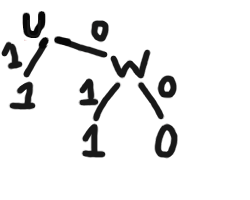
\includegraphics{tree.png}
        the first node is $U$ if  $U = 1$ return 1. Then check $W$ is $W$ is 1 return 1 else return 0.
    \item To create a tree of depth 0.we must not make any decisions thus we must prune all possible first picks, thus
        we pick $\epsilon > \frac{1}{5}(2\log(\frac{5}{2}) + 3\log(\frac{5}{3}) - \log(3) - 2\log(\frac{3}{2})$ which ensures that no split may take place.
        The decision of this tree would always be 1, so in this case it would return 1.
    \end{enumerate}
\end{solution}

\section{Problem 2}
\begin{solution}

    \begin{enumerate}
        \item For each test point i will list the nearest neighbors
            \begin{enumerate}
                \item 1\\
                    \[
                        - \rightarrow -  \;\text{correct}
                    .\] 
                \item 2
                    \[
                        - \rightarrow - \; \text{incorrect}
                    .\] 
                \item 3
                    \[
                        - \rightarrow - \; \text{incorrect}
                    .\] 
                \item 4
                    \[
                        + \rightarrow + \; \text{correct}
                    .\] 
                \item 
                    \[
                        + \rightarrow + \; \text{incorrect}
                    .\] 
            \end{enumerate}
            the test error is $0.6$ which is worse than random picking.
        \item for  $k=1$ we list out the location of the nearest neighbor and its sign and correct vs incorrect
            \begin{enumerate}
                \item 1
                    \[
                        (2,7) \rightarrow + \; \text{incorrect}
                    .\] 
                \item 2
                    \[
                        (5,9) \rightarrow + \; \text{correct}
                    .\] 
                \item 3
                    \[
                        (8,3) \rightarrow - \; \text{incorrect}
                    .\] 
                \item 4
                    \[
                        (8,4) \rightarrow + \; \text{correct}
                    .\] 
                \item 5
                    \[
                        (8,8) \rightarrow - \; \text{correct}
                    .\] 
            \end{enumerate}
            for a total test error of $0.4$
        \item since the dataset is small and sparse using large values of $k$ might include too much noise.
            Using small values of $k$ will also reduce the accuracy because many different points are close to each other.
    \end{enumerate}
\end{solution}
\section{Problem 3}

\section{Problem 4}


\end{document}
